Een ander model is het Spine-Leaf model, Two-Tier-model, waarbij er maar twee lagen switches zijn. In situaties waarbij er veel server naar server communicatie is heeft dit systeem zijn voordelen (East-West traffic). Het gaat dan om veel verkeer binnen een datacenter

\begin{figure}[H]
\centering
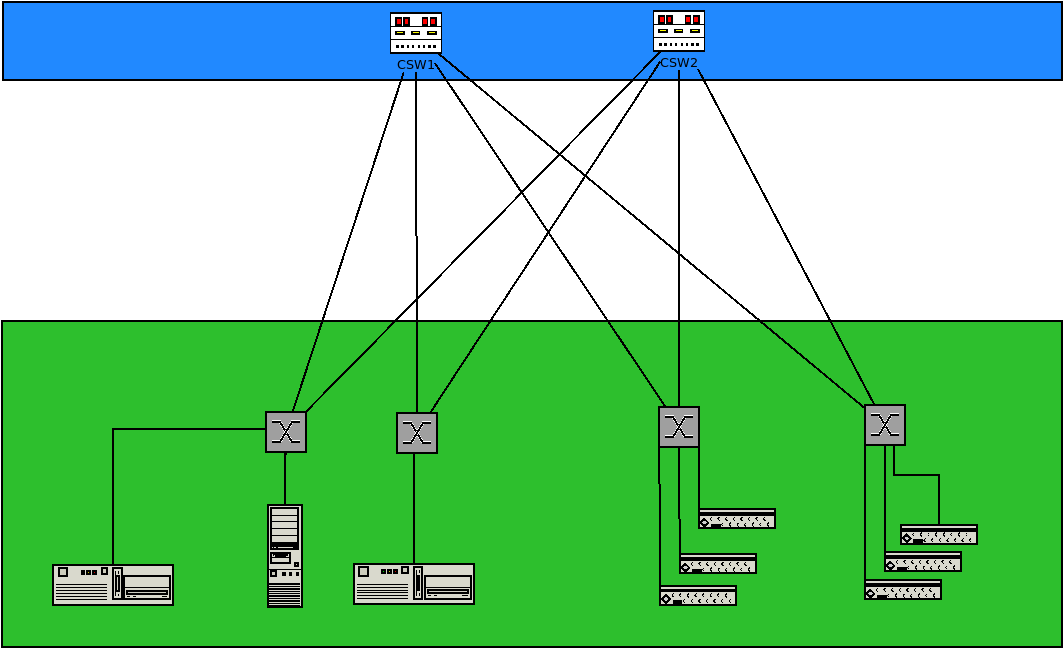
\includegraphics[width=\linewidth]{SpineLeaf.png}
\caption{Blauw is de spine, groen is de leafes laag en rood is de access laag}
\label{SpineLeaf}
\end{figure}

De spine-switches zijn switches met een hoge throughput, lage latency en met poorten die een high-speed verbinding hebben met de leaf-switches.

De leaf-switches zijn de feitelijke Top-of-Rack (TOR) switches met 24 of 48 poorten, maar met een zeer snelle uplink naar de spine-switches.

Voordelen van het two-tier model ten opzicht van het three-tier model:
\begin{itemize}
\item Geen spanning-tree nodig, daar elke spine-switch verbonden is met alle leaf-switches en er geen loops gecre\"eerd kunnen worden
\item Tussen de servers in het datacenter zitten maximaal 2 hops, wat resulteert in een lage latency.
\end{itemize}

Nadelen van het two-tier model ten opzicht van het three-tier model:
\begin{itemize}
\item Doordat elke spine switch met elke leaf switch verbonden moet zijn, is er meer kabel nodig naar de acces (leaf) laag.
\end{itemize}
